\documentclass[20pt]{beamer}

\usetheme{Berkeley}
\setbeamertemplate{caption}[numbered]
\everymath=\expandafter{\the\everymath\displaystyle}

\ifdefined\pdftexversion\else  % non-pdftex case.
	\usepackage{fontspec}
\fi
\makeatletter\@ifpackageloaded{underscore}{}{\usepackage[strings]{underscore}}\makeatother

\newcommand{\diff}[1]{\operatorname{d}#1}
\renewcommand{\vec}[1]{\boldsymbol{#1}}


\author{Henry Ding}
\date{\today}
\title{Lesson 2: Motion in One Dimension}


\begin{document}

\frame{\titlepage}

\begin{frame}
	\frametitle{Homework Questions?}
\end{frame}

\section{Position}


\begin{frame}
	\frametitle{Reference Frames}
	\begin{figure}[ht]
		\centering
		\inkfig{0.8\textwidth}{referenceframe}
		%\caption{}
		\label{fig:referenceframe}
	\end{figure}
	\begin{definition}
		Motion must be defined relative to a \textbf{reference frame}.
	\end{definition}
	\begin{definition}
		A \textbf{coordinate system} in each reference frame specifies position, velocity, acceleration, etc.
	\end{definition}
\end{frame}

\begin{frame}
	\frametitle{Coordinate System}
	\begin{figure}[ht]
		\centering
		\inkfig{0.6\textwidth}{coordinatesystem}
		%\caption{}
		\label{fig:coordinatesystem}
	\end{figure}
\end{frame}

\begin{frame}
	\frametitle{Position and Displacement}
	\begin{figure}[ht]
		\centering
		\inkfig{0.7\textwidth}{positiondisplacement}
		%\caption{}
		\label{fig:positiondisplacment}
	\end{figure}

	\begin{definition}
		\textbf{Position} is a vector pointing from the \textbf{origin} of the coordinate system.
		\textbf{Displacement} is the change in position from one location to another
		\begin{align*}
			\Delta \vec{d}_{AB} = \vec{d}_B - \vec{d}_A.
		\end{align*}
	\end{definition}

	\begin{alertblock}{$\Delta$ Prefix}
		In the sciences, $\Delta$ often represents a change in something.
	\end{alertblock}
\end{frame}

\begin{frame}
	\frametitle{Displacement vs. Distance}
	\begin{figure}[ht]
		\centering
		\inkfig{0.7\textwidth}{distancedisplacement}
		%\caption{}
		\label{fig:distancedisplacement}
	\end{figure}
	\begin{definition}
		\textbf{Distance} is a scalar equal to the total length of the path between two locations, which means distance is always positive. It is not the same as displacement!
	\end{definition}

	\begin{example}
		What is the displacement from $\langle \SI{-3}{\meter}, \SI{2}{\meter} \rangle$ to $\langle \SI{0}{\meter}, \SI{4}{\meter} \rangle$? What distance is covered traveling in a straight line between those two points?
	\end{example}
\end{frame}

\section{Velocity}

\begin{frame}
	\frametitle{Average and Instantaneous Velocity}
	\begin{definition}
		\textbf{Average velocity} is the total displacement $\Delta \vec{d}$ between two points divided by the time $\Delta t$ taken to travel between those points:
		\begin{align*}
			\vec{v}_\mathrm{avg} = \frac{\Delta \vec{d}}{\Delta t} = \frac{\vec{d}_f - \vec{d}_i}{t_f - t_i}.
		\end{align*}
	\end{definition}

	\begin{itemize}
		\item $\vec{v}_\mathrm{avg}$ is a vector parallel to $\Delta \vec{d}$, which shows the direction of movement. The magnitude $||\vec{v}_\mathrm{avg}||$ tells you the rate of movement.
		\item $\vec{v}_\mathrm{avg}$ tells us about average movement, not the finer details!
	\end{itemize}

	\begin{figure}[ht]
		\centering
		\inkfig{0.6\textwidth}{averagevelocity}
		%\caption{}
		\label{fig:averagevelocity}
	\end{figure}
\end{frame}

\begin{frame}
	\frametitle{Instantaneous Velocity}
	\begin{figure}[ht]
		\centering
		\inkfig{\textwidth}{instantaneousvelocity}
		%\caption{}
		\label{fig:instantaneousvelocity}
	\end{figure}
	\begin{definition}
		When the displacement $\Delta \vec{d}$ becomes infinitely small, the average velocity describes the \textbf{instantaneous velocity} $\vec{v}$. $\vec{v}$ is a vector describing the rate and direction of motion at a specific point.
	\end{definition}
\end{frame}

\begin{frame}
	\frametitle{Average Speed}
	\begin{definition}
		\textbf{Average speed} is the total distance $d$ between two points divided by time $\Delta t$ taken to travel between those points:
		\begin{align*}
			v_\mathrm{avg} = \frac{d}{\Delta t}
		\end{align*}
		Note, $v_\mathrm{avg}$ is a scalar and is always positive. However, in most cases $v_\mathrm{avg} \neq ||\vec{v}_\mathrm{avg}||$, even though both are scalars!
	\end{definition}

	\begin{example}
		Anne finishes a race on a circular race track with radius $\SI{30}{\meter}$ in $\SI{15}{\second}$. From the start to end of the race, what is her (a) average velocity (b) average speed?
	\end{example}
\end{frame}

\begin{frame}
	\frametitle{Instantaneous Speed}
	\begin{definition}
		\textbf{Instantaneous speed} $v$ is the average speed $v_\mathrm{avg}$ as the two points become infinitely close to each other. Turns out, this is just the magnitude of the instantaneous velocity $\vec{v}$
		\begin{align*}
			v = ||\vec{v}||.
		\end{align*}
	\end{definition}
	\begin{figure}[ht]
		\centering
		\inkfig{0.8\textwidth}{instantaneousspeed}
		%\caption{}
		\label{fig:instantaneousspeed}
	\end{figure}
	\begin{example}
		Anne finishes a race on a circular race track with radius $\SI{30}{\meter}$ in $\SI{15}{\second}$. If travels at a uniform speed (her instantaneous speed is constant throughout the track), then her Instantaneous speed is always equal to her average speed.
	\end{example}
\end{frame}

\section{Acceleration}

\begin{frame}
	\frametitle{Acceleration}
	\begin{definition}
		\textbf{Average acceleration} is the change in instantaneous velocity $\Delta \vec{v} = \vec{v}_f - \vec{v}_i$ divided by the time taken $\Delta t$
		\begin{align*}
			a_\mathrm{avg} = \frac{\Delta \vec{v}}{\Delta t}.
		\end{align*}
	\end{definition}

	\begin{definition}
		\textbf{Instantaneous acceleration} $a$ is the average acceleration as the time change $\Delta t$ becomes infinitely small.
	\end{definition}

	\begin{itemize}
		\item Acceleration has units of (meter / second) / second or $\SI{}{\meter / \second^2}$.
	\end{itemize}

	\begin{example}
		Andrea changes from an initial velocity of $\langle \SI{5}{\meter/\second}, \SI{-1}{\meter/\second}\rangle$ to a final velocity of $\langle \SI{3}{\meter/\second}, \SI{12}{\meter/\second} \rangle$ in $\SI{10}{\second}$. What is her average acceleration?
	\end{example}
\end{frame}

\section{Graphs}

\begin{frame}
	\frametitle{Position vs. Time Graphs}
	\begin{figure}[t]
		\centering
		\inkfig{0.8\textwidth}{1dvector}
		%\caption{}
		\label{fig:1dvector}
	\end{figure}
	In one dimension, vectors only have one component along a single axis. We can just work with scalars that can be any sign.
	\begin{itemize}
		\item \textbf{note}: to distinguish between distance and position, we will use $x$ for position in one dimension.
	\end{itemize}
	\begin{figure}[b]
		\centering
		\inkfig{0.5\textwidth}{labeled-xt}
		%\caption{}
		\label{fig:labeled-xt}
	\end{figure}
\end{frame}

\begin{frame}
	\begin{theorem}[Slope on a Position vs. Time Graph]
		The slope on a $x(t)$ graph gives the instantaneous velocity as the time interval becomes infinitely small.
	\end{theorem}
	\frametitle{Position vs. Time Graph Example}
	\begin{example}
		Consider the following $x(t)$ graph. Determine the instantaneous velocities at (a) $t = \SI{2}{\second}$ (b) $t = \SI{17}{\second}$. Determine the average velocities from (c) $t =\SI{0}{\second}$ to $t = \SI{10}{\second}$ (d) $t = \SI{0}{\second}$ to $t = \SI{20}{\second}$.
		\begin{figure}[b]
			\centering
			\mplfig{example-xt.pgf}
			%\caption{}
			\label{fig:}
		\end{figure}
	\end{example}
\end{frame}

\begin{frame}
	\frametitle{Velocity vs. Time Graphs}
	$v(t)$ graphs tell us the instantaneous velocity at different times.

	\begin{example}
		Consider the following $v(t)$ graph. Determine the instantaneous acceleration at (a) $t = \SI{2}{\second}$ (b) $t = \SI{7}{\second}$. What is the average acceleration from $t = \SI{0}{\second}$ to $t = \SI{10}{\second}$?

		\begin{figure}[ht]
			\centering
			\mplfig{linear-vt.pgf}
			%\caption{}
			\label{fig:linear-vt}
		\end{figure}
	\end{example}

	\begin{theorem}[Slope on a Velocity vs. Time Graph]
		The slope on a $v(t)$ graph gives instantaneous acceleration.
	\end{theorem}
\end{frame}

\begin{frame}
	\frametitle{Velocity vs. Time Graph Example}
	\begin{example}
		Consider the following $v(t)$ graph. Determine the average velocity from $t = \SI{0}{\second}$ to $t = \SI{10}{\second}$. What is the displacement from $t = \SI{0}{\second}$ to $t = \SI{10}{\second}$?
		\begin{figure}[b]
			\centering
			\mplfig{uniform-vt.pgf}
			%\caption{}
			\label{fig:uniform-vt}
		\end{figure}
	\end{example}
	The rectangular \textit{area} under a $v(t)$ graph gives the displacement!
\end{frame}

\begin{frame}
	\frametitle{Area Under Velocity vs. Time Graph}
	For velocity varying with time, split up the graph into rectangles.
	\begin{figure}[b]
		\centering
		\mplfig{general-vt.pgf}
		%\caption{}
		\label{fig:general-vt}
	\end{figure}
	Each rectangle has area $v(t) \Delta t = \Delta d$, so the whole area is total displacement.
	\begin{theorem}
		The area under a $v(t)$ graph for a time interval is equal to the displacement during that interval.
	\end{theorem}
\end{frame}

\begin{frame}
	\frametitle{Area Under Velocity vs. Time Graph Example}
	\begin{example}
		Find the total displacement for the following $v(t)$ graph from $t = \SI{0}{\second}$ to $t = \SI{10}{\second}$. What is the average velocity from this time interval? Qualitatively graph the position $x(t)$.
		\begin{figure}[t]
			\centering
			\mplfig{area-example-vt.pgf}
			%\caption{}
			\label{fig:area-example-vt}
		\end{figure}
	\end{example}
\end{frame}

\begin{frame}
	\frametitle{Another Velocity vs. Time Graph Example}
	\begin{example}
		A biker is at $x = 0$ at $t = 0$. Graph the biker's position $x(t)$ given $v(t)$:
		\begin{figure}[t]
			\centering
			\mplfig{xt-vt.pgf}
			%\caption{}
			\label{fig:xt-v}
		\end{figure}
	\end{example}
\end{frame}

\begin{frame}
	\frametitle{Motion with Constant Acceleration}
	We will often deal with situations involving constant acceleration, so that the instantaneous acceleration $a$ is the same value at all times. Recall then that the slope on a $v(t)$ graph is always constant. In other words, our $v(t)$ graph is a straight line.
	\begin{example}
		Consider the following graph. Find the constant acceleration $a$.
		\begin{figure}[ht]
			\centering
			\mplfig{constant-a.pgf}
			%\caption{}
			\label{fig:constant-a}
		\end{figure}
	\end{example}
\end{frame}

\begin{frame}
	\frametitle{Average Velocity with Constant Acceleration}
	\begin{example}
		Consider the following graph. Find the average velocity $v_\mathrm{avg}$ from $t_i$ to $t_f$.
		\begin{figure}[ht]
			\centering
			\mplfig{constant-a.pgf}
			%\caption{}
			\label{fig:avg-velocity}
		\end{figure}
	\end{example}
\end{frame}

\begin{frame}
	\frametitle{Displacement with Constant Acceleration}
	\begin{example}
		Consider the following graph. Find the displacement from $t_i$ to $t_f$.
		\begin{figure}[ht]
			\centering
			\mplfig{constant-a.pgf}
			%\caption{}
			\label{fig:displacement}
		\end{figure}
	\end{example}
\end{frame}

\begin{frame}
	\frametitle{Displacement given Initial, Final Velocities}
	\begin{theorem}[Kinematic Formulas]
		For constant acceleration
		\begin{align}
			v_f            & = v_i + at \label{eq:vat}                                                \\
			v_\mathrm{avg} & = \frac{v_i + v_f}{2}                                                    \\
			\Delta x       & = v_\mathrm{avg} t = \left(\frac{v_i + v_f}{2}\right) t \label{eq:xvavg} \\
			\Delta x       & = v_i t + \frac{1}{2}at^2
		\end{align}
	\end{theorem}
	However, note from Eq.~\eqref{eq:vat}
	\begin{align*}
		t = \frac{v_f - v_i}{a},
	\end{align*}
	so from Eq.~\eqref{eq:xvavg}
	\begin{align*}
		\Delta x                  & = \left(\frac{v_i + v_f}{2}\right) \left(\frac{v_f - v_i}{a}\right) \\
		\Rightarrow v_f^2 - v_i^2 & = 2a \Delta x.
	\end{align*}
\end{frame}

\begin{frame}
	\frametitle{Constant Acceleration Example}
	\begin{example}
		A boat accelerates from $\SI{0}{\meter/\second}$ to $\SI{8}{\meter/second}$ in $\SI{5}{\second}$. What is the boat's (a) acceleration (b) average velocity (c) displacement?
	\end{example}

	\begin{example}
		A train, initially moving at $\SI{-3}{\meter/\second}$ accelerates at a rate of $\SI{2}{\meter/second}$ over $\SI{4}{\meter}$. What is the train's final velocity? How long does it take the train to accelerate to this final velocity?
	\end{example}
\end{frame}

\begin{frame}
	\frametitle{Free Fall}
	Objects near the surface of the Earth fall towards the ground with an acceleration of around $g = \SI{9.81}{\meter/\second^2}$.
	\begin{example}
		Donna throws a ball straight up at $\SI{5}{\meter/\second}$. How long does it take for (a) the ball to stop moving (b) the ball to return to Donna. Approximate $g = \SI{10}{\meter/\second^2}$.
	\end{example}

	\begin{example}
		Maria drops a ball from a cliff of height $\SI{80}{\meter}$ above the ground. How long does it take for the ball to reach the ground? What is the ball's velocity when it hits the ground? Approximate $g = \SI{10}{\meter/\second^2}$.
	\end{example}

	\begin{example}
		Marie throws a ball straight up at $\SI{3}{\meter/\second}$ on a cliff of height $\SI{30}{\meter}$ above the ground. How long does it take for the ball to fall to the ground? Use $g = \SI{9.81}{\meter/\second^2}$
	\end{example}
\end{frame}

\section{Homework 2}

\begin{frame}
	\frametitle{Homework Conventions}
	When solving physics problems,
	\begin{itemize}
		\item Define variables for numbers.
		      \begin{itemize}
			      \item[ex.] ``Let $x_f = \SI{5.0}{\meter}, x_i = \SI{3.0}{\meter}, \Delta t = \SI{2.0}{\second}$.''
		      \end{itemize}
		\item Solve symbolically using variables.
		      \begin{itemize}
			      \item[ex.] ``$v_\mathrm{avg} = (x_f - x_i) / \Delta t$.''
		      \end{itemize}
		\item Plug in numbers only \textit{at the end} to find your answer.
		      \begin{itemize}
			      \item[ex.] ``$v_\mathrm{avg} = (\SI{5.0}{\meter} - \SI{3.0}{\meter}) / \SI{2.0}{\second} = \SI{1.0}{\meter/\second}$.''
		      \end{itemize}
	\end{itemize}
	\begin{alertblock}{Why?}
		\begin{enumerate}
			\item \textit{Speed}: it's faster to write $a, x$ than write out $\SI{9.81}{\meter/\second}$ or $\SI{4.82}{\meter}$.
			\item \textit{Accuracy}: it's easier to mistake $4.0$ for $4.6$, but harder to write $x$ instead of $v$. Also, it's easier to plug everything into a calculator once at the end, instead of constantly using the calculator for every step of the problem.
		\end{enumerate}
	\end{alertblock}
	For excellent tips on general problem solving strategies, I highly recommend checking out \href{https://bpb-us-e1.wpmucdn.com/sites.harvard.edu/dist/0/550/files/2023/11/problemschap1.pdf}{this chapter} by Harvard lecturer David Morin. (Warning: the reading is quite long and assumes some more advanced math/physics knowledge, but the main ideas should be accessible.)
\end{frame}


\begin{frame}
	\frametitle{Homework 2}
	\begin{block}{Textbook Problems}
		\begin{itemize}
			\item \href{https://openstax.org/books/physics/pages/3-concept-items}{OpenStax Physics (High School) Chapter 3 Concept Items} 3, 15
			\item \href{https://openstax.org/books/physics/pages/3-problems}{OpenStax Physics (High School) Chapter 3 Problems} 12, 15
			\item \href{https://openstax.org/books/physics/pages/3-multiple-choice}{OpenStax Physics (High School) Chapter 3 Multiple Choice Test Prep} 18, 19, 25, 26
		\end{itemize}
	\end{block}
	\begin{block}{
			\href{https://www.wiley.com/en-us/Physics\%2C+Volume+1\%2C+5th+Edition-p-9780471320579}{\textit{Physics}, Volume 1, 5th Edition, Chapter 2 Multiple Choice 10}}
		An object is tossed vertically into the air with an initial velocity of $\SI{8}{\meter/\second}$. Using the sign convention up is positive, how does the vertical component of the acceleration $a_y$ of the object (after leaving the hand) vary during the flight of the object?
		\begin{enumerate}
			\item[(a)] On the way up $a_y > 0$, on the way down $a_y < 0$.
			\item[(b)] On the way up $a_y < 0$, on the way down $a_y > 0$ .
			\item[(c)] On the way up $a_y > 0$, on the way down $a_y < 0$.
			\item[(d)] On the way up $a_y < 0$, on the way down $a_y < 0$.
		\end{enumerate}
	\end{block}
\end{frame}

\begin{frame}
	\frametitle{Homework 2}
	\begin{block}{\textit{Physics}, Volume 1, 5th Edition, Chapter 2 Exercise 13}
		The minute hand of a wall clock measures 11.3 cm from axis to tip. What is the displacement vector of its tip (a) from a quarter after the hour to half past, (b) in the next half hour, and (c) in the next hour?
	\end{block}

	\begin{block}{\textit{Physics}, Volume 1, 5th Edition, Chapter 2 Exercise 31, 32}
		How far does the runner whose velocity-time graph is shown in Fig. 2-34 travel in $\SI{16}{\second}$? What is the acceleration of the runner at $t = \SI{11}{\second}$?
		\begin{figure}[ht]
			\centering
			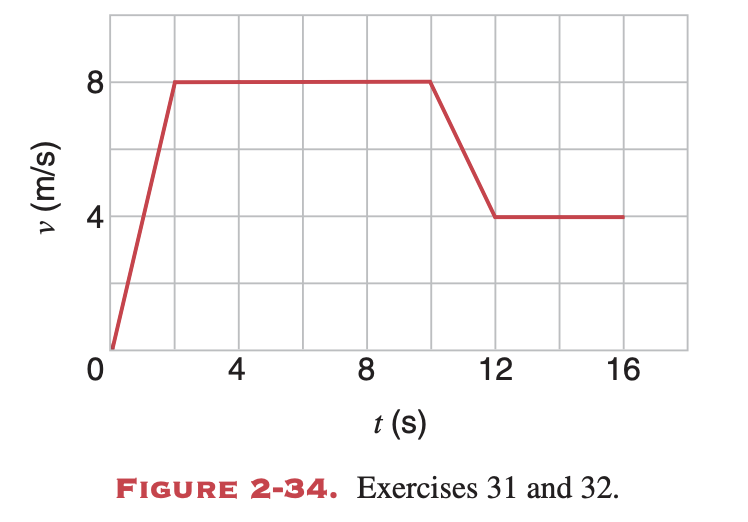
\includegraphics[width=0.5\textwidth]{runnerproblem.png}
			%\caption{}
			\label{fig:runnerproblem}
		\end{figure}
	\end{block}
\end{frame}

\end{document}
